\begin{tikzpicture}[node distance=2cm and 1.5cm]

\node (asv) [yellowbox] {Yellowfin Surfzone ASV1};

\node (img) [left=2cm of asv] {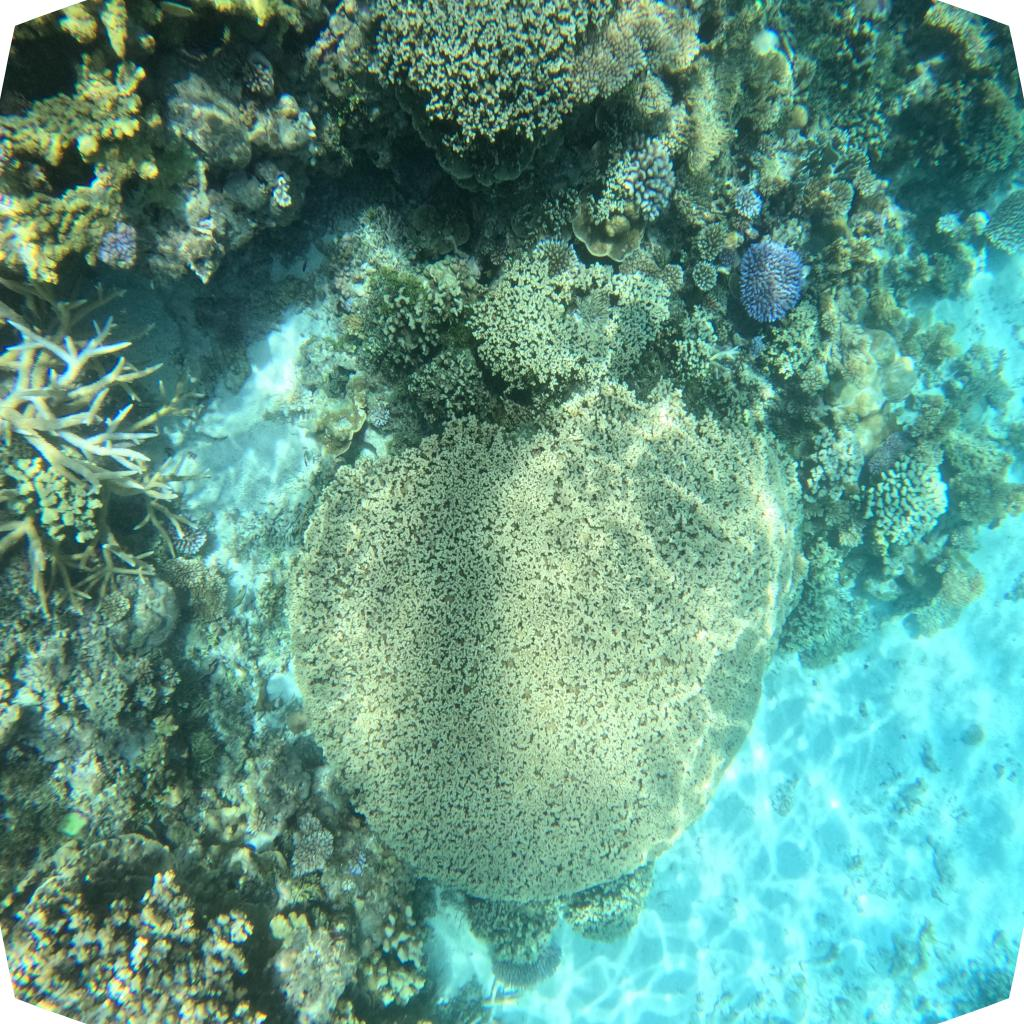
\includegraphics[width=3cm]{fig4a.jpg}};

\node (meta) [right=2cm of asv] {
    \adjustbox{max width=8cm}{
    \begin{tabular}{@{}lrrrrrrr@{}}
    \toprule
    Filename & Lat & Lon & N\_UTM & E\_UTM & Depth & Temp \\
    \midrule
    GPAB2912 & 7.18 & 171 & 793850 & 513200 & -1.92 & 31.4 \\
    GPAB2913 & 7.18 & 171 & 793852 & 513198 & -1.93 & 31.4 \\
    GPAB2914 & 7.18 & 171 & 793854 & 513195 & -1.94 & 31.4 \\
    GPAB2915 & 7.18 & 171 & 793855 & 513193 & -1.94 & 31.4 \\
    GPAB2916 & 7.18 & 171 & 793857 & 513190 & -1.95 & 31.4 \\
    \bottomrule
    \end{tabular}
    }
};

\draw [arrow] (asv.west) -- node[above] {Images} (img.east);
\draw [arrow] (asv.east) -- node[above] {Metadata} (meta.west);

\node (augment) [below=1cm of img, redbox] {Segmentation Augmentation};
\node (augimg) [below=1cm of augment] {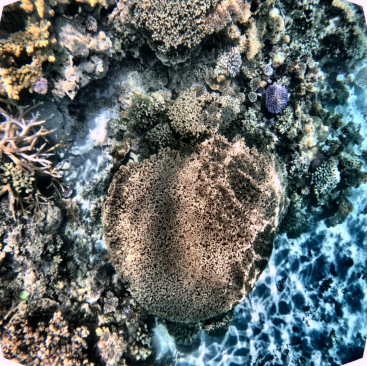
\includegraphics[width=3cm]{fig4b.png}};

\begin{scope}[on background layer]
    \draw [arrow] (img) -- (augimg);
\end{scope}

\node (large) [right=2cm of augimg, yshift=1.75cm, bluecircle] {Large SAM2\\Mask Proposal\\Model};
\node (small) [right=2cm of augimg, yshift=-1.75cm, bluecircle] {Small SAM2\\Mask Proposal\\Model};

\node (allmasks) [right=6cm of augimg, minimum width=3.2cm, minimum height=1.2cm, draw=none, align=center, graybox] {All Mask\\Proposals};

\draw [arrow] (augimg.east) -- ++(0.5cm, 0) coordinate (branch)
    |- (large.west);
\draw [arrow] (branch) |- (small.west);

\draw [arrow] (large.east) -- ++(0.5cm,0) |- ([yshift=0.3cm]allmasks.west);
\draw [arrow] (small.east) -- ++(0.5cm,0) |- ([yshift=-0.3cm]allmasks.west);

\node (cropcenter) [right=2cm of allmasks, yshift=0cm] {};

\node (crop1) [above=2.25cm of cropcenter] {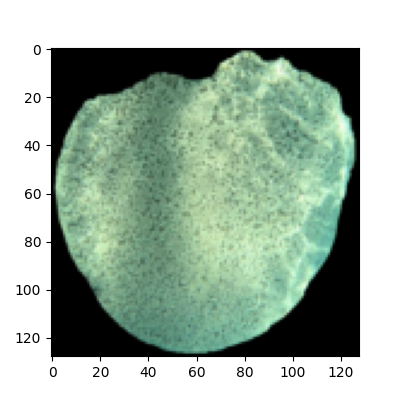
\includegraphics[width=1.4cm]{fig4c.png}};
\node (crop2) [below=0.05cm of crop1] {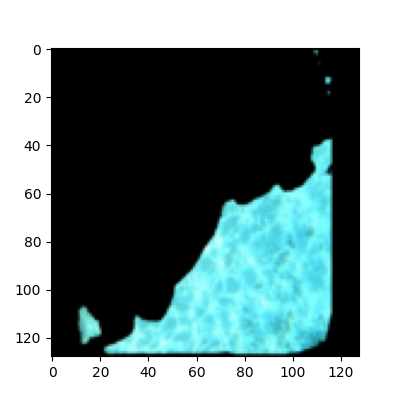
\includegraphics[width=1.4cm]{fig4d.png}};
\node (dots)  [below=0.05cm of crop2] {\Large$\vdots$};
\node (crop3) [below=0.05cm of dots] {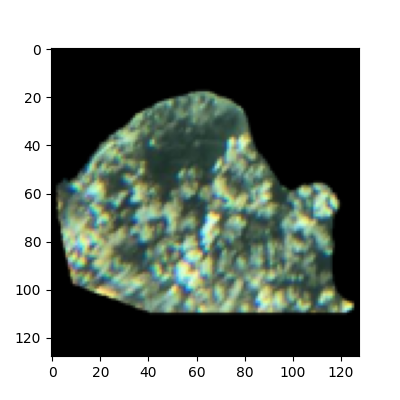
\includegraphics[width=1.4cm]{fig4e.png}};
\node (crop4) [below=0.05cm of crop3] {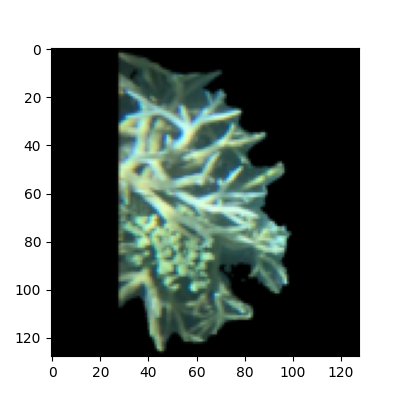
\includegraphics[width=1.4cm]{fig4f.png}};

\draw [arrow] (allmasks.east) -- ++(1cm, 0);

\draw [decorate, decoration={brace, amplitude=6pt}, thick]
    ([xshift=0mm]crop1.north west) -- ([xshift=0mm]crop1.north east)
    node [midway, above=6pt] {$\sim$200 ($N$) Mask Proposals};

\coordinate (vectorcenter) at ($(crop1)!0.5!(crop4)$);
\node (maskaug) [right=2cm of vectorcenter, redbox, align=center] {Mask\\Preprocessing};
\coordinate (augcenter) at ($(maskaug.east) + (2cm,0cm)$);

\node (aug1) [above=2.125cm of augcenter] {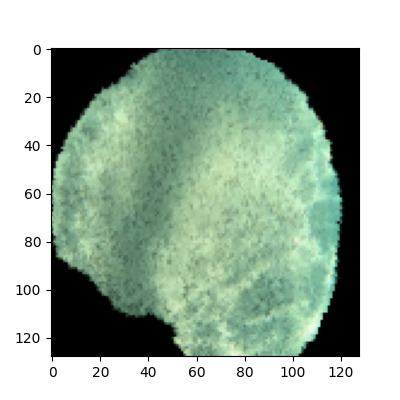
\includegraphics[width=1.4cm]{fig4g.png}};
\node (aug2) [below=0.05cm of aug1] {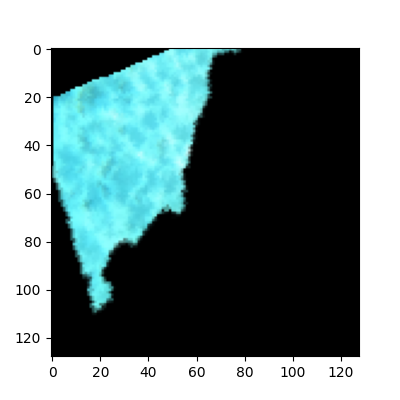
\includegraphics[width=1.4cm]{fig4h.png}};
\node (augdots) [below=0.05cm of aug2] {\Large$\vdots$};
\node (aug3) [below=0.05cm of augdots] {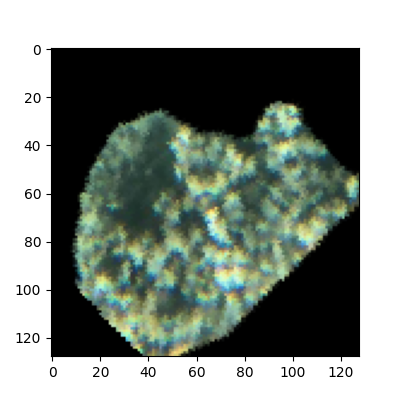
\includegraphics[width=1.4cm]{fig4i.png}};
\node (aug4) [below=0.05cm of aug3] {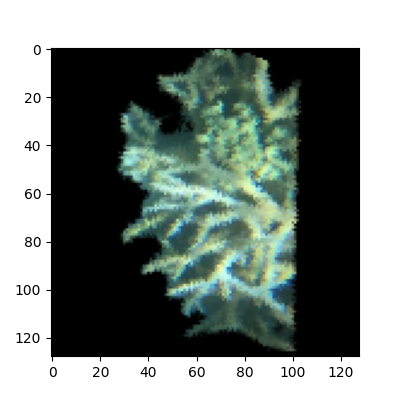
\includegraphics[width=1.4cm]{fig4j.png}};

\coordinate (augvectorcenter) at ($(aug1)!0.5!(aug4)$);

\begin{scope}[on background layer]
    \draw[arrow]
        ([xshift=0.5cm]crop1.east |- vectorcenter) --
        ([xshift=-0.5cm]aug1.west |- augvectorcenter);
\end{scope}

\begin{scope}[every path/.style={>=stealth, ->, thick, gray!50}]
    \draw (crop1.east) -- (aug1.west);
    \draw (crop2.east) -- (aug2.west);
    \draw (crop3.east) -- (aug3.west);
    \draw (crop4.east) -- (aug4.west);
\end{scope}

\node (cnn1) [right=3.5cm of augvectorcenter, yshift=1.5cm, bluecircle] {};
\node (cnn2) [right=1.2cm of cnn1, bluecircle] {};
\node (cnndots) [right=1.2cm of cnn2] {$\cdots$};
\node (cnnM) [right=1.2cm of cnndots, bluecircle] {};

\foreach \i in {1,2,3,4} {
    \foreach \j in {1,2,M} {
        \draw[arrow, bend left=15, looseness=1.1, draw=gray!30] (aug\i.east) to (cnn\j.west);
    }
}

\draw [decorate, decoration={brace, amplitude=6pt, raise=3pt}, thick]
    (cnn1.north west) -- (cnnM.north east)
    node [midway, above=8pt] {CNN Submodels ($M$)};

\tikzset{
    resnet/.style = {rectangle, rounded corners=8pt, minimum size=1.4cm, draw=none, fill=blue!20},
    fc/.style = {circle, minimum size=0.6cm, draw=black, fill=green!20, inner sep=1pt},
    pipelinearrow/.style = {dashed, thick, ->, >=stealth, shorten <=-1pt}
}

\foreach \j/\x in {1/1.5cm, 2/0cm, M/-1.5cm} {
    \draw[pipelinearrow]
        (cnn\j.south) -- ++(0,-0.85cm) coordinate (line\j)
        -- ($(line\j)+(0,-1.4cm)$) node[resnet] (resnet\j) {BB}
        -- ($(resnet\j.south)+(0,-0.6cm)$) node[fc] (fc\j) {FC}
        -- ++(0,-2.25cm);

    \node[resnet] at ($(line\j)+(0,-1.4cm)$) {BB};
    \node[fc] at ($(resnet\j.south)+(0,-0.6cm)$) {FC};
}

\tikzstyle{logitdot} = [circle, minimum size=0.2cm, inner sep=0pt, draw=black!50, fill=gray!50]

\foreach \j/\shift in {1/0.2, 2/0.15} {
    \foreach \k in {0,1,2,3,4} {
        \foreach \i in {1,...,17} {
            \pgfmathparse{int(mod(\i+\j+\k, 5))}
            \edef\shade{\pgfmathresult}
            \node[logitdot, fill=gray!\shade0]
                at ($(fc\j.south) + (\k*0.05cm,-2cm - \i*0.25cm + \k*0.05cm)$) {};
        }
    }

    \node[anchor=north, font=\tiny] at ($(fc\j.south) + (0,-6.65cm)$) {$(N \times K)$};
}

\node at ($(fc2)!0.5!(fcM) + (0,-4cm)$) {$\cdots$};

\foreach \j in {0,1,2, 3,4} {
    \foreach \i [count=\k from 0] in {1,...,17} {
        \pgfmathparse{int(mod(\k+\j, 5))}
        \edef\shade{\pgfmathresult}
        \node[logitdot, fill=gray!\shade0]
            at ($(fcM.south) + (\j*0.05cm,-2cm - \i*0.25cm + \j*0.05cm)$) {};
    }
}
\node[anchor=north, font=\tiny] at ($(fcM.south) + (0,-6.65cm)$) {$(N \times K)$};

\coordinate (stackstart) at ($(fcM.south) + (-0.25cm,-2.25cm)$);
\coordinate (stackend) at ($(stackstart) + (0,-4.25cm)$);

\draw[arrow, thin]
    ($(stackend) + (3pt,-6pt)$) -- ++(0.6cm, 0.6cm)
     node[midway, below=2pt, font=\tiny] {$N$};

\draw[decorate, decoration={brace, mirror, amplitude=6pt}]
    ($(stackstart) + (0cm,0.2cm)$) --
    ($(stackend) + (0cm,0cm)$)
    node[midway, xshift=-11pt, font=\tiny] {$K$};

\coordinate (first-logit) at ($(fc1.south) + (-0.25cm,-2.25cm)$);
\coordinate (logit-center) at ($(fc1.south)!0.5!(fcM.south) + (0,-2.5cm)$);

\node (ensemble) [bluecircle] at ($(first-logit) + (-4cm,-1.6cm)$)
    {Ensemble\\Model};

\draw[arrow, draw=gray!50]
  ($(logit-center) + (-3.5cm, -2.5cm)$)
    to[out=180, in=0, looseness=1.2]
  (ensemble.east);

\draw[arrow, draw=gray!50]
  ($(logit-center) + (-1.25cm, -0.6cm)$)
    to[out=180, in=0, looseness=1.2]
  (ensemble.east);

\draw[arrow, draw=gray!50]
  ($(logit-center) + (2.35cm, -2.6cm)$)
    to[out=180, in=0, looseness=1.2]
  (ensemble.east);

\node (softmax) [right=0.5cm of ensemble, smallredbox, align=center] {\small $\text{Softmax}(\cdot)$\\\tiny$(N\times M\times K)$};

\coordinate (ensemblelogits) at ($(ensemble.west) + (-2cm,2.4cm)$) -- (logit-center);

\coordinate (logitgrid-center) at ($(fcM.south) + (0,-2cm - 2.125cm)$);

\coordinate (logitgrid-left) at ($(logitgrid-center) + (-0.35cm,0)$);

\foreach \i [evaluate=\i as \shade using {int(mod(\i,5))}] in {1,...,17} {
    \node[logitdot, fill={\ifnum\i=5 red!80\else gray!\shade0\fi}]
        at ($(ensemblelogits) + (-3.5cm,-3.5-0.25*\i cm)$) {};
}

\draw[black] ($(ensemblelogits) + (-3.35,-0.2cm)$) rectangle
              ($(ensemblelogits) + (-3.65,-4.55cm)$);

\draw[arrow] (ensemble.west) -- node[midway, above] {$\hat{\bm{p}}_i=\sum_{m=1}^M\hat{\alpha}_m\cdot\tilde{\bm{p}}_m$}
    ($(ensemblelogits) + (-3cm,-2.4cm)$);

\foreach \i/\label in {     1/{branching\_acropora:bleached},
2/{branching\_acropora:healthy},
3/{finger\_acropora:bleached},
4/{finger\_acropora:healthy},
5/{finger\_porites:bleached},
6/{finger\_porites:healthy},
7/{knob\_porites:bleached},
8/{knob\_porites:healthy},
9/{mounding\_:bleached},
10/{mounding\_:healthy},
11/{noncoral},
12/{oddball:bleached},
13/{oddball:healthy},
14/{pocillopora\_:bleached},
15/{pocillopora\_:healthy},
16/{table\_acropora:bleached},
17/{table\_acropora:healthy} }
{
\ifnum\i=5
    \node[anchor=east, font=\scriptsize, fill=yellow!50, rounded corners, inner sep=1pt]
        at ($(ensemblelogits) + (-3.65cm,-2.75-0.25cm*\i)$) {\texttt{\label}};
\else
    \ifnum\i=11
        \node (noncorallabel) [anchor=east, font=\scriptsize, fill=red!50, rounded corners, inner sep=1pt]
            at ($(ensemblelogits) + (-3.65cm,-2.75-0.25cm*\i)$) {\texttt{\label}};
    \else
        \node[anchor=east, font=\scriptsize]
            at ($(ensemblelogits) + (-3.65cm,-2.75-0.25cm*\i)$) {\texttt{\label}};
    \fi
\fi
}

\node[anchor=north, font=\tiny]
    at ($(ensemblelogits) + (-3.5cm, 0.25 cm)$) {$(N \times K)$};

\node (reject) [redoctagon, above left=1.5cm and 4cm of noncorallabel] {Reject\\Noncoral\\Masks};
\draw[arrow, bend left=25, thick, red!70]
    (noncorallabel.west) to (reject.south east);

\node (consolidation) [bluecircle, left=14cm of ensemble] {Mask\\Consolidation};

\draw[arrow, black]
    ($(consolidation.east) + (4cm, 0)$) --
    ($(consolidation.east) + (0.2cm, 0)$);

\node (segmap) [left=1.5cm of consolidation, yshift=-3.5cm] {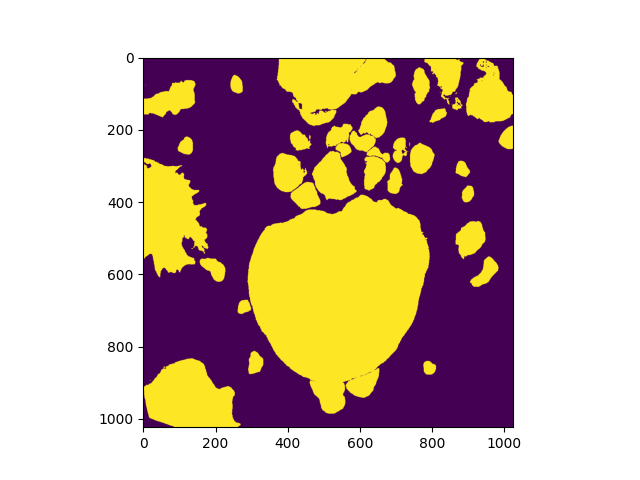
\includegraphics[width=5cm]{fig4k.png}};

\draw[arrow, bend right=25] (consolidation.west) to node[midway, yshift=3mm, above] {Segmentation Map} (segmap.north);

\node (stats) [graybox, right=3.5cm of segmap.east, anchor=west, align=center, text width=4.5cm]
    {Compute Statistics:\\Coral Cover by Genus \& Bleaching};

\draw[arrow] (segmap.east) -- ([xshift=-5pt]stats.west);

\node (newdata) [right=2.5cm of stats, align=center] {
    \begin{tikzpicture}[scale=1.5, baseline=-1.5ex]
        \fill[gray!30] (0,0) ellipse (0.5cm and 0.15cm);
        \fill[gray!30] (-0.5,0) -- (-0.5,-1.0) arc (180:360:0.5cm and 0.15cm) -- (0.5,0);
        \fill[gray!50] (0,-1.0) ellipse (0.5cm and 0.15cm);

        \foreach \y in {0,-0.25,-0.5,-0.75} {
            \draw[gray!60] (-0.5,\y) arc (180:360:0.5cm and 0.15cm);
        }

        \draw[gray!60] (0,0) ellipse (0.5cm and 0.15cm);
        \draw[gray!60] (-0.5,0) -- (-0.5,-1.0);
        \draw[gray!60] (0.5,0) -- (0.5,-1.0);

        \node[above, yshift=2mm] at (0,0.2) {New Data};
    \end{tikzpicture}
};

\draw[arrow] ([xshift=3pt]stats.east) -- ([xshift=-5pt]newdata.west);

\draw[arrow, thick, gray!50, bend left=40]
    ([xshift=4pt]meta.east) to
    node[pos=0.9, above, sloped, font=\scriptsize, black] {Join by Image ID}
    ([xshift=4pt]newdata.east);

\end{tikzpicture}
